\documentclass{article}
\usepackage[margin=1in]{geometry}
\usepackage{amsmath,amsthm,amssymb}
\usepackage{bbm,enumerate,mathtools}
\usepackage{tikz,pgfplots}
\usepackage{chessboard}
\usepackage[hidelinks]{hyperref}
\usepackage{multicol} % Problem 35
\usepackage{xstring} % Difficulty command
\usetikzlibrary{shapes.geometric}

\newenvironment{question}{\begin{trivlist}\item[\textbf{Question.}]}{\end{trivlist}}
\newenvironment{note}{\begin{trivlist}\item[\textbf{Note.}]}{\end{trivlist}}
\newenvironment{references}{\begin{trivlist}\item[\textbf{References.}]}{\end{trivlist}}
\newenvironment{related}{\begin{trivlist}\item[\textbf{Related.}]\end{trivlist}\begin{enumerate}}{\end{enumerate}}

\newcommand\score[1]{
\pgfmathsetmacro\pgfxa{#1+1}
\tikzstyle{scorestars}=[
  star,
  star points=5,
  star point ratio=2.25,
  draw,
  inner sep=3pt,
  anchor=outer point 5
]
  \begin{tikzpicture}[baseline]
    \draw[opacity=0] (0,-0.5) rectangle (0,0.2); % Workaround for whitespace at the bottom.
    \foreach \i in {1,...,4} {
      \pgfmathparse{(\i<=#1?"yellow":"gray")}
      \edef\starcolor{\pgfmathresult}
      \draw (\i*4.5ex,0) node[name=star\i,scorestars,fill=\starcolor]  {};
    }
  \end{tikzpicture}
}

\newcommand{\difficulty}[1]{%
  \IfEqCase{#1}{%
      {1}{
        
\begin{tikzpicture}[scale=0.7, baseline=0.9mm]%
          \definecolor{slopegreen}{rgb}{0.0, 0.5, 0.0}%
          \fill[slopegreen] (0.5,0.5) circle (0.5);%
        \end{tikzpicture}%
      }%
      {2}{
        
\begin{tikzpicture}[scale=0.7, baseline=0.9mm]%
          \definecolor{slopeblue}{rgb}{0.0, 0.44, 1.00}
          \fill[slopeblue] (0,0) rectangle (1,1);%
        \end{tikzpicture}%
      }%
      {3}{
\begin{tikzpicture}[scale=0.7, baseline=0.9mm]\fill (0,0.5)--(0.5, 0)--(1,0.5)--(0.5,1)--cycle; \end{tikzpicture}}%
      {4}{
\begin{tikzpicture}[scale=0.7, baseline=0.9mm]\fill (0.25,0)--(0,0.5)--(0.25,1)--(0.5,0.5)--cycle; \fill (0.75,0)--(0.5,0.5)--(0.75,1)--(1,0.5)--cycle;\end{tikzpicture}}%
      % you can add more cases here as desired
  }[\PackageError{difficulty}{Undefined difficulty level: #1}{}]%
}%
\newcommand{\rating}[2]{\difficulty{#1}\\\score{#2}\\}


\begin{document}
  Consider a peaceable queens problem in an $n \times n \times n$ chess
  ``cube'', where a queen can move in any diagonal direction.
  \begin{figure}[ht!]
    \centering
    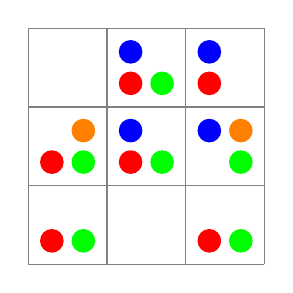
\begin{tikzpicture}
      \draw [gray] (0,0) grid (3, 3);
      \node at (0.5, 2.5) {\Huge \textcolor{red}{\symqueen}};
      \node at (1.5, 0.5) {\Huge \textcolor{black!20!green}{\symqueen}};
      \foreach \x/\y/\c in {
        0.3/0.3/red, 0.3/1.3/red, 1.3/1.3/red, 1.3/2.3/red, 2.3/0.3/red, 2.3/2.3/red,
        0.7/0.3/green, 0.7/1.3/green, 1.7/1.3/green, 1.7/2.3/green, 2.7/0.3/green, 2.7/1.3/green,
        1.3/1.7/blue, 1.3/2.7/blue, 2.3/1.7/blue, 2.3/2.7/blue,
        0.7/1.7/orange, 2.7/1.7/orange}
      {
        \fill[\c] (\x, \y) circle (0.15cm);
      }
    \end{tikzpicture}\hspace{0.5cm}
    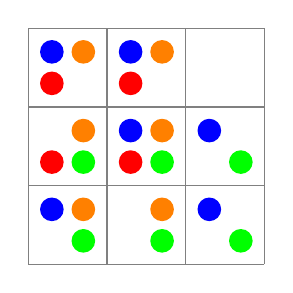
\begin{tikzpicture}
      \draw [gray] (0,0) grid (3, 3);
      \node at (2.5, 2.5) {\Huge \textcolor{blue}{\symqueen}};
      \foreach \x/\y/\c in {
        0.3/1.3/red, 0.3/2.3/red, 1.3/1.3/red, 1.3/2.3/red,
        0.7/0.3/green, 0.7/1.3/green, 1.7/0.3/green, 1.7/1.3/green, 2.7/0.3/green, 2.7/1.3/green,
        0.3/0.7/blue, 0.3/2.7/blue, 1.3/1.7/blue, 1.3/2.7/blue, 2.3/0.7/blue, 2.3/1.7/blue,
        0.7/0.7/orange, 0.7/1.7/orange, 0.7/2.7/orange, 1.7/0.7/orange, 1.7/1.7/orange, 1.7/2.7/orange}
      {
        \fill[\c] (\x, \y) circle (0.15cm);
      }
    \end{tikzpicture}\hspace{0.5cm}
    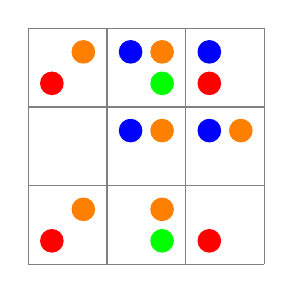
\begin{tikzpicture}
      \draw [gray] (0,0) grid (3, 3);
      \node at (0.5, 1.5) {\Huge \textcolor{orange}{\symqueen}};
      \foreach \x/\y/\c in {
        0.3/0.3/red, 0.3/2.3/red, 2.3/0.3/red, 2.3/2.3/red,
        1.7/0.3/green, 1.7/2.3/green,
        1.3/1.7/blue, 1.3/2.7/blue, 2.3/1.7/blue, 2.3/2.7/blue,
        0.7/0.7/orange, 0.7/2.7/orange, 1.7/0.7/orange, 1.7/1.7/orange, 1.7/2.7/orange, 2.7/1.7/orange}
      {
        \fill[\c] (\x, \y) circle (0.15cm);
      }
    \end{tikzpicture}
    \caption{
      At least four hyper-queens can be placed peaceably on a
      $3 \times 3 \times 3$ board.
    }
  \end{figure}
  \begin{question}
    What is the greatest number of queens that can be placed on an
    $n \times n \times n$ board?
  \end{question}

  \begin{related}
    \item If $n^{k-1}$ queens can be placed on a
      $\displaystyle\underbrace{n \times n \times \hdots \times n}_{k}$ board
      for sufficently large $n$, how large must $n$ be?
  \end{related}
  \begin{references}
    \item \url{https://math.stackexchange.com/q/2232287/121988}
  \end{references}
\end{document}
